\documentclass{article}
\usepackage{tikz}
\usepackage{amsmath}
\usepackage{amsfonts}
\usepackage{amssymb}

\begin{document}

\section{TikZ Diagram Test - Tagged Templates}

\begin{figure}[h]
\centering
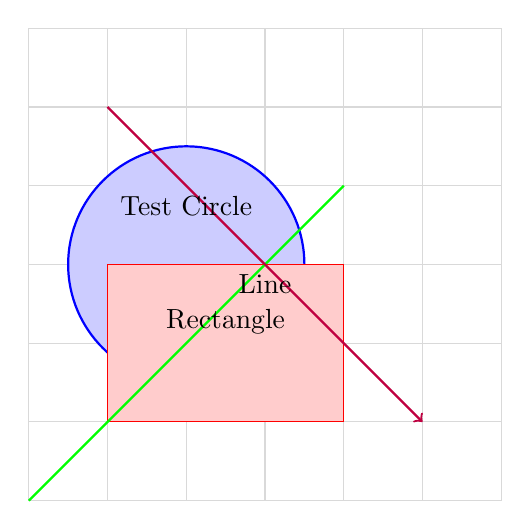
\begin{tikzpicture}[scale=1]
\draw[gray!30][step=1cm] (0,0) grid (6,6);
\draw[fill=blue!20, draw=blue, thick] (2,3) circle (1.5cm);
\draw[fill=red!20, draw=red] (1,1) rectangle (4,3);
\draw[thick, green] (0,0) -- (4,4);
\draw[->, thick, purple] (1,5) -- (5,1);
\node[above] at (2,3.5) {Test Circle};
\node[above] at (2.5, 2) {Rectangle};
\node[below] at (3, 3) {Line};
\end{tikzpicture}
\caption{Test diagram with TikZ components created using tagged templates}
\end{figure}

\end{document}